% *********************************************************************
% © 2021–2026 Jeremy Sylvestre
%
% Permission is granted to copy, distribute and/or modify this document
% under the terms of the GNU Free Documentation License, Version 1.3 or
% any later version published by the Free Software Foundation; with no
% Invariant Sections, no Front-Cover Texts, and no Back-Cover Texts. A
% copy of the license is included in the appendix entitled “GNU Free
% Documentation License” that appears in the output document of this
% PreTeXt source code. All trademarks™ are the registered® marks of
% their respective owners.
%
% *********************************************************************

\newcommand*{\xmin}{-1.5}
\newcommand*{\xmax}{8}
\newcommand*{\ymin}{-1.5}
\newcommand*{\ymax}{4.6}

\begin{tikzpicture}
[
	closedpt/.style={circle,draw,fill,inner sep=0pt,minimum size=4pt},
	openpt/.style={circle,draw,inner sep=0pt,minimum size=4pt}
]

	% axes
	\draw[->,thick] (\xmin,0) -- (\xmax,0) node[below] {$t$};
	\draw[->,thick] (0,\ymin) -- (0,\ymax) node[right] {$y$};

	% graph
	\draw[thick, green!33!black, domain=0.22:7.75, smooth]
	  plot (\x,{ln \x})
	  node[below left] {$\ln(t)$}
	;
	\draw[thick, blue, domain=\xmin:1.5, smooth]
	  plot (\x,{exp \x})
	  node[below right] {$\exp(t)$}
	;

	\draw[dashed,gray,thin] (\xmin,\xmin) -- node[above,sloped,very near end] {$y = t$} (\ymax,\ymax);
	\draw[thick,<->,red] (2,3) -- (3,2);

	% tangent line to logarithm
	\draw (0.5,0.265) -- (7,2.432) node[above] {$m = \dfrac{1}{t^\ast}$};
	\draw[dashed] (3,1.099) -- (3,0) node[below] {$t^\ast$};
	\draw[dashed] (0,0.599) -- (1.5,0.599) -- (1.5,0);
	\draw[dashed] (0,1.765) -- (5,1.765) -- (5,0);
	\draw[|-|] (1.5,-0.6) to node[below] {${\change{t}}$} (5,-0.6);
	\draw[|-|] (-0.25,0.599) to node[left] {${\change{y}}$} (-0.25,1.765);

\end{tikzpicture}
